\section{Messvorgang}
 
In diesem Versuch wird das NanoSurf NaioSTM verwendet, siehe \autoref{fig:naio}.
\begin{figure}
  \centering
  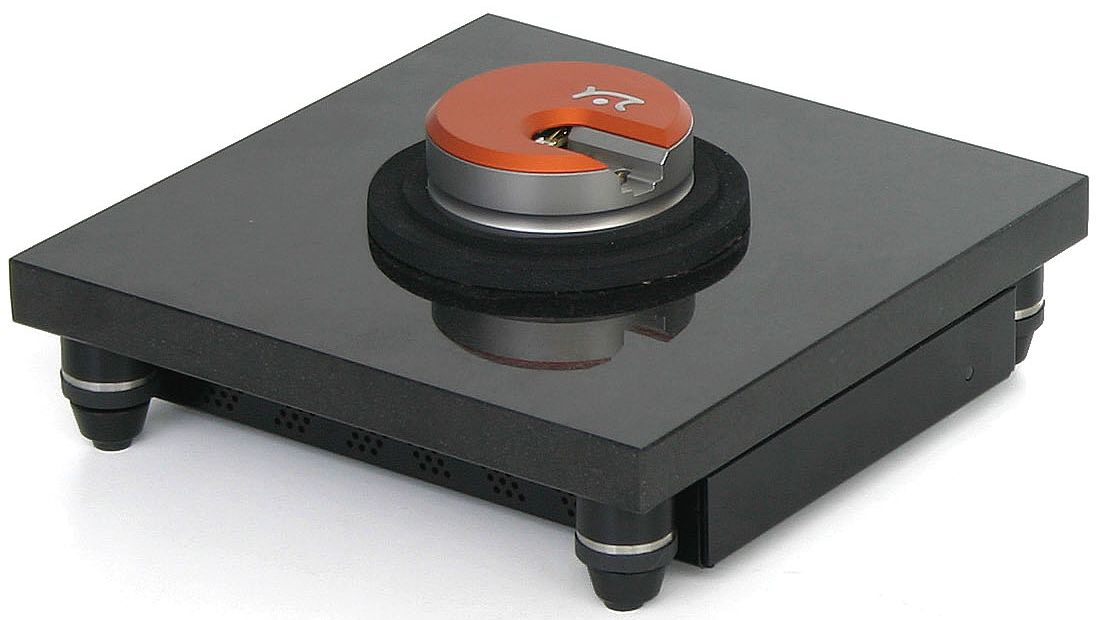
\includegraphics[width=0.8\textwidth]{./images/naiostm-zoom.jpg}
  \caption{%
    NaioSTM von NanoSurf auf der erschütterungsdämpfenden Steinplatte.~\cite{naio}
  }\label{fig:naio}
\end{figure}

Zunächst wird eine Spitze gerissen und in der dafür vorgesehen Halterung befestigt.
Hiernach wird die Probe, die magnetisch auf einem Probenstab gehalten wird, ins Mikroskop eingesetzt.
Der Abstand zwischen Probe und Spitze wird mithilfe der Steuerungssoftware manuell verringert, bis sich beide Objekte beinahe berühren.
Daraufhin wird die automatische Annäherung benutzt, die bis zu einem bestimmten Tunnelstrom auf die Probe zufährt.
Ist diese Annäherung erfolgt, können Aufnahmen erstellt werden.

Für die Aufnahmen von HOPG wird in einem ersten Schritt eine Übersichtsaufnahme mit einer Kantenlänge von ca.\ \SI{200}{\nano\meter} angefertigt.
Nach Auswahl einer geeigneten Stelle wird eine Aufnahme mit einer Kantenlänge von \SI{4.5}{\nano\meter} angefertigt, um die Gitterkonstante und den Korrekturfaktor für die Piezokristalle zu bestimmen.

Für die Aufnahme der Goldoberfläche wird ein Bild mit einer höheren Auflösung von \num{2048} Linien und einer Kantenlänge von \SI{400}{\nano\meter} angefertigt.
